% !TeX root = ../FFY_graduate.tex

% \chapter{研究方法}
\chapter{基于手势描述的协同手势生成算法研究}
\label{sec:GG} 
本章将详细介绍一种描述驱动的协同手势生成框架(如图\ref{fig:teaser}所示)。
首先,我们提出了一种统一的运动表示方法,将不同来源的运动数据嵌入到紧凑的潜在空间中(第\ref{sec:method:m_rep}节)。在此基础上,我们设计了一种可控的手势潜在扩散模型(第\ref{sec:method:gld}节),该模型包含两个关键组件:
(1) 一个手势变分自编码器,用于学习手势的低维潜在表示;
(2) 一个在该潜在空间中高效运行的分层条件扩散模型。
为了实现语义和节奏的协同精确控制,我们提出了一种手势描述框架(第\ref{sec:method:caption}节),该框架利用运动-语言模型为手势数据生成描述性文本标注,填补了手势数据描述性文本标注的空白。
此外,我们还设计了一种多粒度描述控制机制(第\ref{sec:method:control}节)以确保精确的语义注入。

\begin{figure*}[!h]
  \centering
  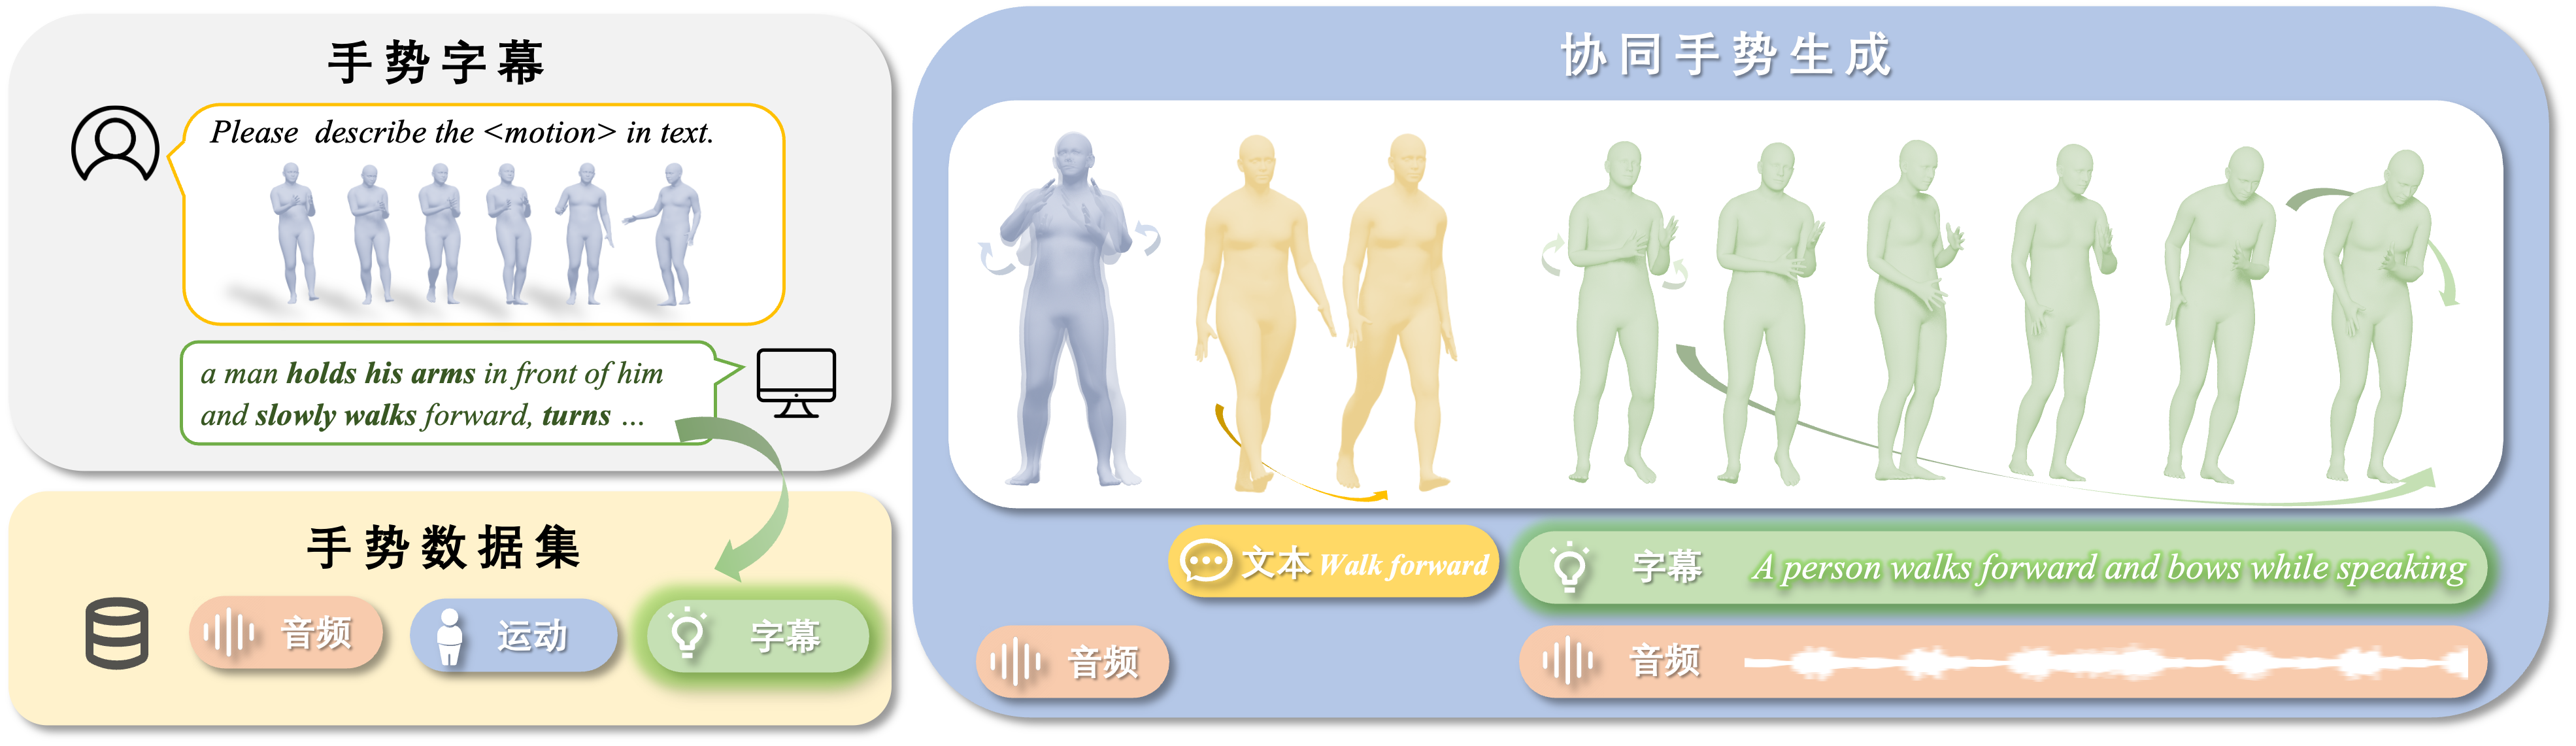
\includegraphics[width=\linewidth]{teaser.png}
  \caption{\textbf{CoordSpeaker} 支持 \textit{手势字幕} 和定制的 \textit{协同的说话者动作生成},既能与字幕保持语义一致,又能与音频保持节奏同步。例如,在演讲场景中,我们的方法允许说话者在讲话时自然地向前走并鞠躬,无缝地做出结束手势。} %Our method generates natural speaking gestures synchronized with speech and text captions. Given speech and text prompts (such as ``sitting'', ``waving while talking'', etc.), our model produces coordinated gesture motions that align with both speech rhythm and textual semantics. The figure above demonstrates gesture examples generated under the same speech with different text prompts.}
  \label{fig:teaser}
\end{figure*}

\section{运动表示}
\label{sec:method:m_rep}
为了将不同来源的运动数据统一到紧凑的潜在空间中,我们实现了一种紧凑的运动表示方法。首先将各种数据格式转换为统一的HumanML3D格式表示,然后通过我们的运动编码器$\mathcal{E}$(在第\ref{sec:method:gld}节中描述)将其映射到一个具有代表性的潜在空间。
% [freetalker: ...->humanml3d]
% We expect that the features of the different motion datasets are correctly preserved. In contrast to [16] and [17], where [16] represents human motions with discrete codes and [17] retargets human motion to a homograph consisting of five terminal joints (head, hands, and feet), potentially losing important detailed information such as shoulders and fingers, our approach addresses this issue and preserves motion details. We first convert the rotation matrix of the motion capture (BVH format) data to an axis angle representation of SMPL-X [20]. For the 3D position dataset, we fit it to the SMPL-X representation using VPoser [20]. We then scale the 3D translations of the root joint appropriately and adjust the initial orientation to be uniform across the different datasets as [17]. With the SMPL-X model forward computation, we can obtain the 3D position of the SMPL-X representation. Then as in [21], we use root height, root linear and rotational velocity, joint rotation, joint position, joint velocity, and foot contact as kinematic feature representations. Each frame of the processed motion sequence has 659 dimensional features, which we denote as xˆ0 ∈ RTM ×659, where TM denotes the number of motion sequence frames.

\subsection{统一运动表示}
\label{sec:method:m_rep:unified}
% 22joints->nfeats=263(用于输入motionllm生成description), 55joints->nfeats=659(用于输入gld训练)
% [mld] HumanML3D Format [17] proposes a motion representation x1:L inspired by motion features in character control [66, 45, 65]. This redundant representation is quite suited to neural models, particularly variational autoencoders. Specifically, the i-th pose xi is defined by a tuple of root angular velocity r ̇a ∈ R along Y-axis, root linear velocities (r ̇x, r ̇z ∈ R) on XZ-plane, root height ry ∈ R, local joints positions jp ∈ R3Nj , velocities jv ∈ R3Nj and rotations jr ∈ R6Nj in root space, and binary foot-ground contact features cf ∈ R4 by thresholding the heel and toe joint velocities, where Nj denotes the joint number, giving:  xi = {r ̇a, r ̇x, r ̇z, ry, jp, jv, jr, cf }.
为了利用额外人体运动数据集中的语义先验知识,我们采用HumanML3D~\cite{guo2022humanml3d}并将不同的运动数据统一到一个一致的特征空间中。
参照~\cite{yang2024freetalker,guo2022humanml3d},第$i$帧运动被表示为$x^i=\left\{\dot{r}^a, \dot{r}^x, \dot{r}^z, r^y, \mathbf{j}^p, \mathbf{j}^v, \mathbf{j}^r, \mathbf{c}^f\right\}$,其中$\dot{r}^a, \dot{r}^x, \dot{r}^z, r^y$表示根关节的角速度、线速度和高度,$\mathbf{j}^p, \mathbf{j}^v, \mathbf{j}^r$表示关节位置、速度和旋转,$\mathbf{c}^f$表示足部接触特征。
虽然原始HumanML3D格式遵循SMPL~\cite{loper2023smpl}骨架的22个关节,但本文将其扩展到55个关节以更好地适应手势数据。因此,每一帧运动被表示为659维特征向量,记为$x \in \mathbb{R}^{T\times 659}$,其中$T$为序列长度。


\subsection{潜在表示}
近期研究表明,潜在表示在神经运动建模中发挥着关键作用[]。
本文采用基于Transformer的VAE模型将运动序列编码到紧凑且信息丰富的潜在空间中,该模型由编码器$\mathcal{E}$和解码器$\mathcal{D}$组成,并通过长跳跃连接来保持运动细节。
具体而言,运动序列$x^{1:L}$首先通过编码器$\mathcal{E}$编码为潜在向量$z \in \mathbb{R}^{n\times d}$,其中$d$表示潜在维度。编码器接收逐帧运动特征和可学习的分布令牌作为输入,生成运动潜在空间的高斯分布参数$\mu$和$\sigma$。这些参数通过标准VAE采样过程重参数化得到潜在向量。
对于运动解码,$\mathcal{D}$采用带有交叉注意力机制的Transformer架构。它以零运动令牌作为查询,潜在向量$z$作为键和值,生成重建的运动序列$\hat{x}^{1:L}$。整个VAE通过均方误差(MSE)和Kullback-Leibler(KL)散度的组合进行训练:
\begin{equation}
L_{\text{VAE}} = \|x^{1:L} - \hat{x}^{1:L}\|_2^2 + \beta \text{KL}(q_{\phi}(z|x^{1:L})\|p(z))
\label{eq:loss_vae}
\end{equation}
其中$\beta$平衡重建和正则化项。这种潜在表示方法在保持运动保真度和多样性的同时实现了高效的手势合成。
% [mld] Latent Format [40]. Latent representations are widely used in neural models [46, 47, 19, 9]. We recognize it as motion representation in latent space. By leveraging VAE models, latent vectors can represent plausible motions as:  xˆ1:L = D(z), z = E(x1:L)
% [mld: ...->latents]
% We build our motion Variational AutoEncoder, V, based on a transformer-based architecture [46], which consists of a transformer encoder E and a transformer decoder D. The motion VAE, V = {E, D}, is trained by the motion x1:L reconstruction only with the Mean Squared Error (MSE) loss and the Kullback-Leibler (KL) loss. We further enhance two transformers [70] of E and D with long skip connections [59], and remove the action biases used in [46]. The encoder could produce a representative, low-dimensional latent space with high informative density, and the decoder could well reconstruct the latent into motion sequences. More specifically, the motion encoder E takes as input learnable distribution tokens, and frame-wise motion features x1:L of arbitrary length L. We use the embedded distribution tokens as Gaussian distribution parameters μ and σ of the motion latent space Z to reparameterize [30] latent z ∈ Rn×d whose dimension is similar to [46]. The motion decoder D relies on the architecture of the transformer decoder with cross attention mechanism, which takes the L number of zero motion tokes as queries, a latent z ∈ Rn×d as memory, and finally, generates a human motion sequence xˆ1:L with L frames. According to [47], both the latent space Z and variable durations help the model to produce more diverse motions. To further enhance the latent representation, we leverage a long skip-connection structure for the transformer-based encoder E and decoder D. We also explore the effectiveness of the latent’s dimensions on motion sequences representation in Tab. 4. Hence, our VAE models present a stronger motion reconstruction ability and richer diversity (cf. Tab. 5 and Tab. 6). We provide more details about the architecture and the training in the supplementary.

% [syntalker] 3.2 Motion Representation Module  Motion encoding. Recent studies in motion generation have demonstrated that vector-quantized autoencoder (VQ-VAE) [44] possesses a remarkable capability for compressing motion information [2, 17, 55]. We also utilize vector quantization for motion encoding. Following [17, 33, 54], we use a residual VQ-VAE (RVQ-VAE) as the quantization layer. To further decrease the coupling between body parts, we segment the body into three parts: upper body, fingers, and lower body, like in [2, 28], and train a separate RVQ-VAE for each part. In details, the motion sequence M can be represented as m1:N ∈ RN ×D , which is firstly encoded into a latent vector sequence z1:n ∈ Rn×d with downsampling ratio of n/N and latent dimension d, using 1D convolutional encoder E; The z1:n ∈ Rn×d obtained through the encoder then enters the first quantization layer Q1, each vector subsequently finds its nearest code entry in the layer’s codebook C1 = {c1  k }K  k=1 ⊂ Rd to get the  first quantization code ˆz1  1:n, also we can calculate the quantization  residual1:n = ˆz1  1:n − z1:n. The residual1:n then enter the second quantization layer Q2 finds its nearest code entry in the layer’s codebook C2 = {c2  k }K  k=1 ⊂ Rd to get the second quantization code  ˆz21:n. Accordingly, ˆz3  1:n,ˆz4  1:n... can be calculated in this manner. As the last step of motion encoding, we sum all quantization code together to get the final code zˆ = ÍQ  q=1 ˆzv .  Motion decoding. Similar to motion encoding, three separated decoders are introduced for generating corresponding motions for all body parts, which are 1D convolutional decoders. During training, the motion data is encoded with motion encoders and fused with speech and prompt conditions by the diffusion-based conditional generation module, and then passed through the decoders to get the reconstructed motions. During inference, the motion encoder is not utilized, the generated motion is obtained directly from the speech and prompt conditions with the diffusion module and motion decoders.

\begin{figure*}[t]
  \centering
  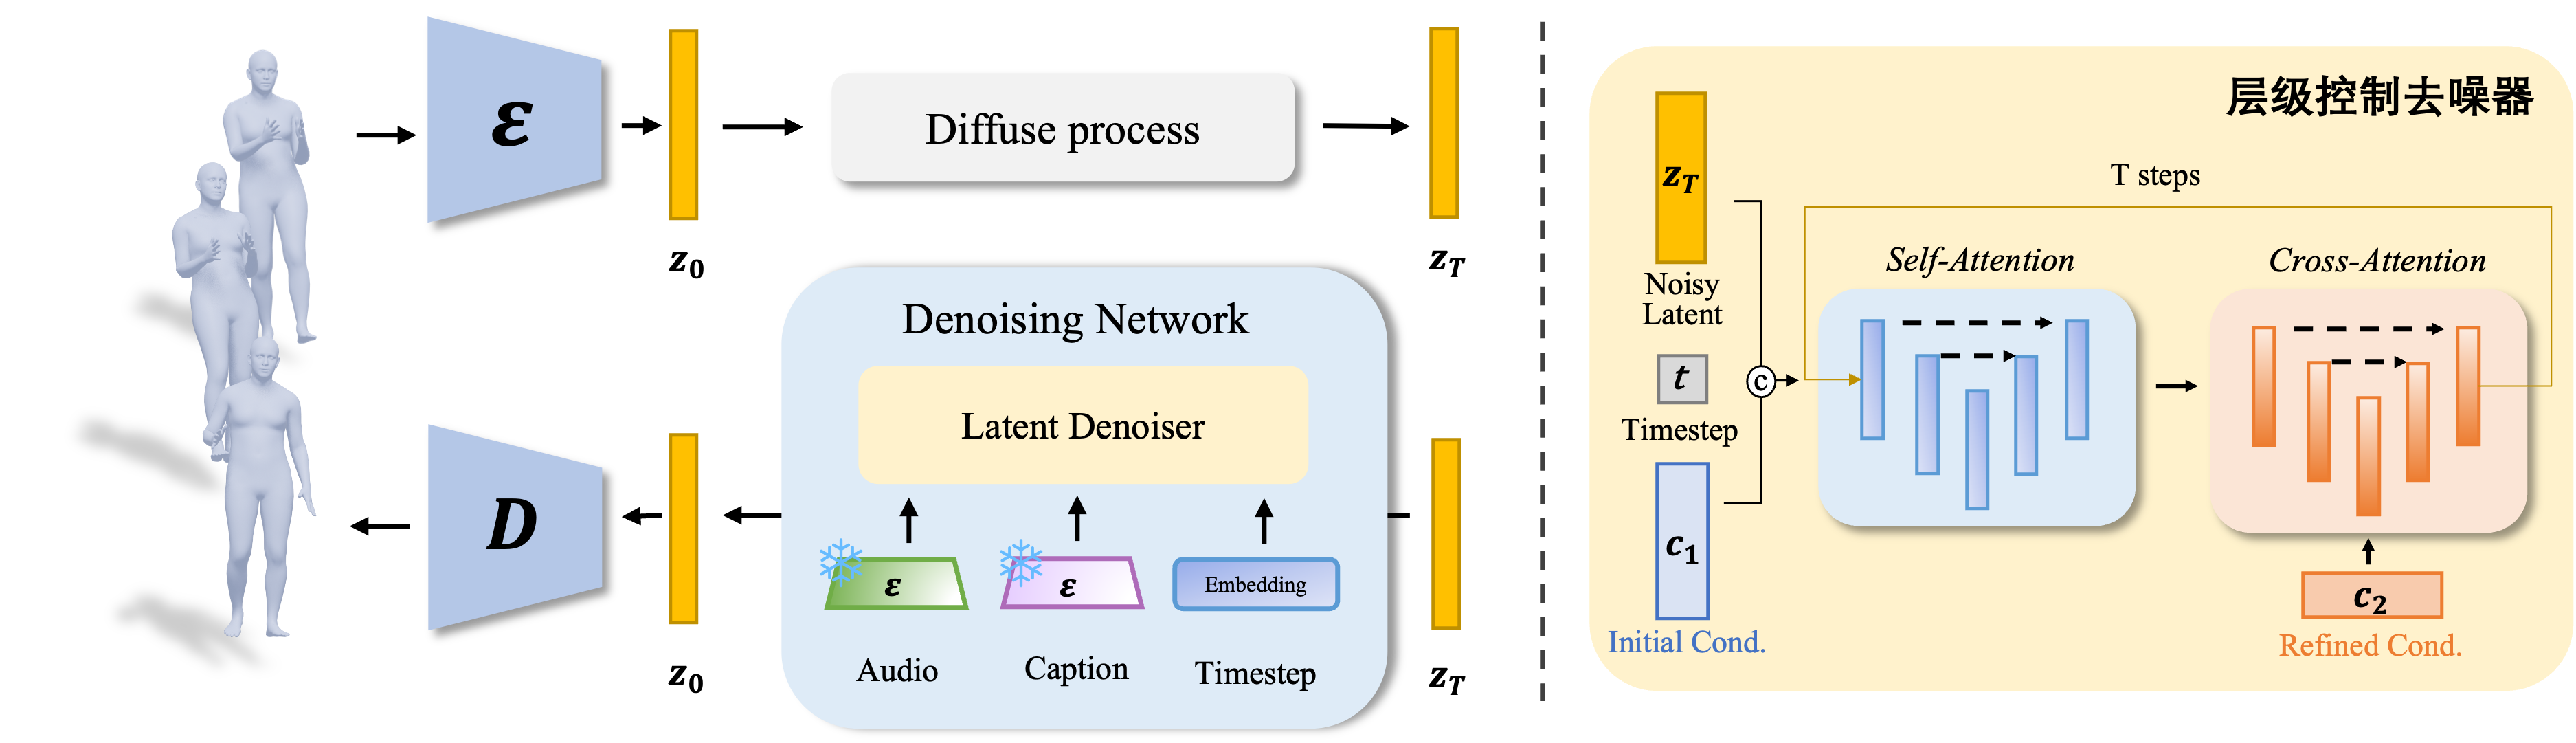
\includegraphics[width=\linewidth]{model_v1_zh.png}
  \caption{协同手势生成模型概览。我们的条件潜在扩散模型(第~\ref{sec:method:gld}节)由两个关键组件组成:(1)手势变分自动编码器,可学习统一的低维潜在表示,从而实现紧凑的跨数据集运动建模,以及(2)分层控制的降噪器,确保分层条件注入并在该学习到的潜在空间中有效运行。}
  \label{fig:method:model}
\end{figure*}
\section{可控手势潜在扩散模型}
\label{sec:method:gld}
% Diffusion model 出于其强大的生成质量与多样性,已经在图像、音频、视频、运动生成等领域取得了显著成果 \cite{}。一些工作在原始运动空间针对运动序列进行diffusion,但存在效率低下与高频噪声的问题\cite{}。我们基于latent space进行diffusion,旨在生成隐变量z∈ Rn×d,可以显著提高效率。
基于VAE学习的紧凑潜在表示,我们提出了一种可控手势潜在扩散模型,用于生成高质量手势。与以前直接在原始运动序列上执行扩散的方法不同,我们的模型通过对潜在向量进行操作,显著降低了计算要求,同时保持了生成质量。
% mld(optional改进)
% 3.2. Motion Latent Diffusion Model  Diffusion probabilistic models [63] can gradually anneal the noise from a gaussian distribution to a data distribution p(x) by learning the noise prediction from a T length Markov noising process, giving {xt}tT=1. It leads to a significant influence in many research domains, such as the most famous image synthesis models [11, 23, 62, 56], the density estimation model [29] and the motion generation models [69, 75]. For motion generation, these works train the diffusion models with a transformer-based denoiser θ (xt, t), which anneal the random noise to motion sequence {xˆ1:N  t }tT=1 iteratively. However, diffusion on raw motion sequences is inefficient and requires exhausting computational resources. Besides, raw motion data from the markless or marker-based motion capture system usually remain high-frequency outliers, which might have a side effect on the diffusion model to learn the actual data distribution. To reduce the computational requirements of the diffusion models on raw motion sequences and improve the synthesized quality, we perform the diffusion process on a representative and lowdimensional motion latent space. Here, we introduce our denoiser θ. Different from the previous UNet-based architecture [59] on the 2D image latent zI , we build a transformer-based denoising model with long skip connections [4] on the motion latent z ∈ Rn×d, which is more suitable for sequential data, like human motion sequences. The diffusion on latent space is modeled as a Markov nosing process using:  q (zt | zt−1) = N (√αtzt−1, (1 − αt) I) .   where the constant αt ∈ (0, 1) is a hyper-parameters for sampling. We then use {zt}tT=0 to denote the noising sequence, and zt−1 = θ (zt, t) for the t-step denoising. We further focus on the unconditional generation with the simple objective [23]:  LMLD := E ,t  [  ‖ − θ (zt, t)‖2  2  ]  , where ∼ N (0, 1), z0 = E(x1:L). During the training of θ, the encoder E is frozen to compress motion into z0. The samples of the diffusion forward process are from the latent distribution p(z0). During the diffusion reverse stage, θ first predict zˆ0 with T iterative denoising steps, then D decodes zˆ0 to motion results with one forward.

\subsection{潜在扩散过程}
潜在空间中的扩散过程遵循马尔可夫链,逐步向潜在向量$\mathbf{z} \in \mathbb{R}^{n\times d}$添加高斯噪声。对于噪声步骤$t \in [1,T]$,前向过程定义为:
\begin{equation}
  q(z_t|z_{t-1}) = \mathcal{N}(\sqrt{\alpha_t}z_{t-1}, (1-\alpha_t)\mathbf{I}),
\end{equation}
其中$\alpha_t \in (0,1)$是常数方差调度,且$z_T \sim \mathcal{N}(0, \mathbf{I})$。
为了生成高质量手势,我们采用基于Transformer的去噪器$\epsilon_\theta$来迭代预测和去除噪声。从随机噪声$z_T$开始,去噪器逐步恢复潜在向量$\hat{z}_0$,然后通过$\mathcal{D}$解码为手势运动。去噪过程同时受音频特征$\mathbf{A}$和描述嵌入$\mathbf{C}$的条件约束。

\subsection{分层条件注入}
为了实现对手势生成的精确多模态控制,我们的模型通过精心设计的嵌入和分层注入过程整合多个条件。
% 我们采用CLIP文本编码器~\cite{radford2021clip}和WavLM编码器~\cite{chen2022wavlm}分别从描述和音频中提取语义特征$\mathbf{C} \in \mathbb{R}^{512}$和声学特征$\mathbf{A} \in \mathbb{R}^{T\times1133}$。提取的特征通过特定模态的嵌入层进一步处理以获得最终的条件嵌入。
对于字幕编码,使用预训练的CLIP文本编码器~\cite{radford2021clip} 提取语义特征 $\mathbf{C} \in \mathbb{R}^{512}$。使用WavLM编码器~\cite{chen2022wavlm} 提取音频特征 $\mathbf{A} \in \mathbb{R}^{T\times1133}$,捕获丰富的声学信息,包括韵律和节奏模式。然后通过特定于模态的嵌入层处理这些原始特征,以形成条件嵌入 $\mathbf{C}$ 和 $\mathbf{A}$。
此外,为了实现更灵活和精确的生成控制,我们提出了一种分层条件注入机制,包含两个阶段(图\ref{fig:method:model}):
首先,初始条件$\mathbf{c_1}$与噪声潜在向量和时间步嵌入串联后输入去噪器$\epsilon_\theta$,提供基本指导。
其次,细化条件$\mathbf{c_2}$通过交叉注意力机制在去噪器内部整合,实现精细的控制调整。

\subsection{无分类器指导}
为了增强生成手势的质量和可控性,我们在训练和推理过程中采用无分类器指导\cite{ho2022classifier}。在训练过程中,随机屏蔽10\%的条件输入以同时学习有条件和无条件分布。在推理过程中,噪声预测通过不同指导的预测加权组合计算:
\begin{equation}
  \begin{split}
      \epsilon_\theta^s(z_t, t, \mathbf{c}) = & s_1 \epsilon_\theta(z_t, t, \mathbf{c}=\{\varnothing, \mathbf{A}\}) \\
      & + s_2 \epsilon_\theta(z_t, t, \mathbf{c}=\{\mathbf{C}, \varnothing\}) \\
      & + (1 - s_1 - s_2) \epsilon_\theta(z_t, t, \mathbf{c}=\{\varnothing, \varnothing\}),
  \end{split}
\end{equation}
其中$s_1$、$s_2$分别是音频和描述的指导尺度,且$s_1, s_2 > 1$可以增强其效果。
这种方法允许对描述和音频分别应用指导,在手势生成过程中实现更精确的条件控制。

\subsection{训练与推理}
潜在扩散模型使用简单的$\ell_2$目标进行训练\cite{ho2020ddpm, chen2023executing}:
\begin{equation}
  \mathcal{L}_{\text{Diff}} = \mathbb{E}_{\epsilon,t}[\|\epsilon - \epsilon_\theta(z_t, t, c)\|_2^2],
\end{equation}
其中$\epsilon \sim \mathcal{N}(0,\mathbf{I})$且$z_0 = \mathcal{E}(x^{1:L})$。在推理过程中,我们的模型首先通过$T$个去噪步骤预测潜在向量$\hat{z}_0$,然后通过解码器$\mathcal{D}$的单次前向传播将其解码为运动序列$\hat{x}^{1:L}$。

\begin{figure*}[t]
  \centering
  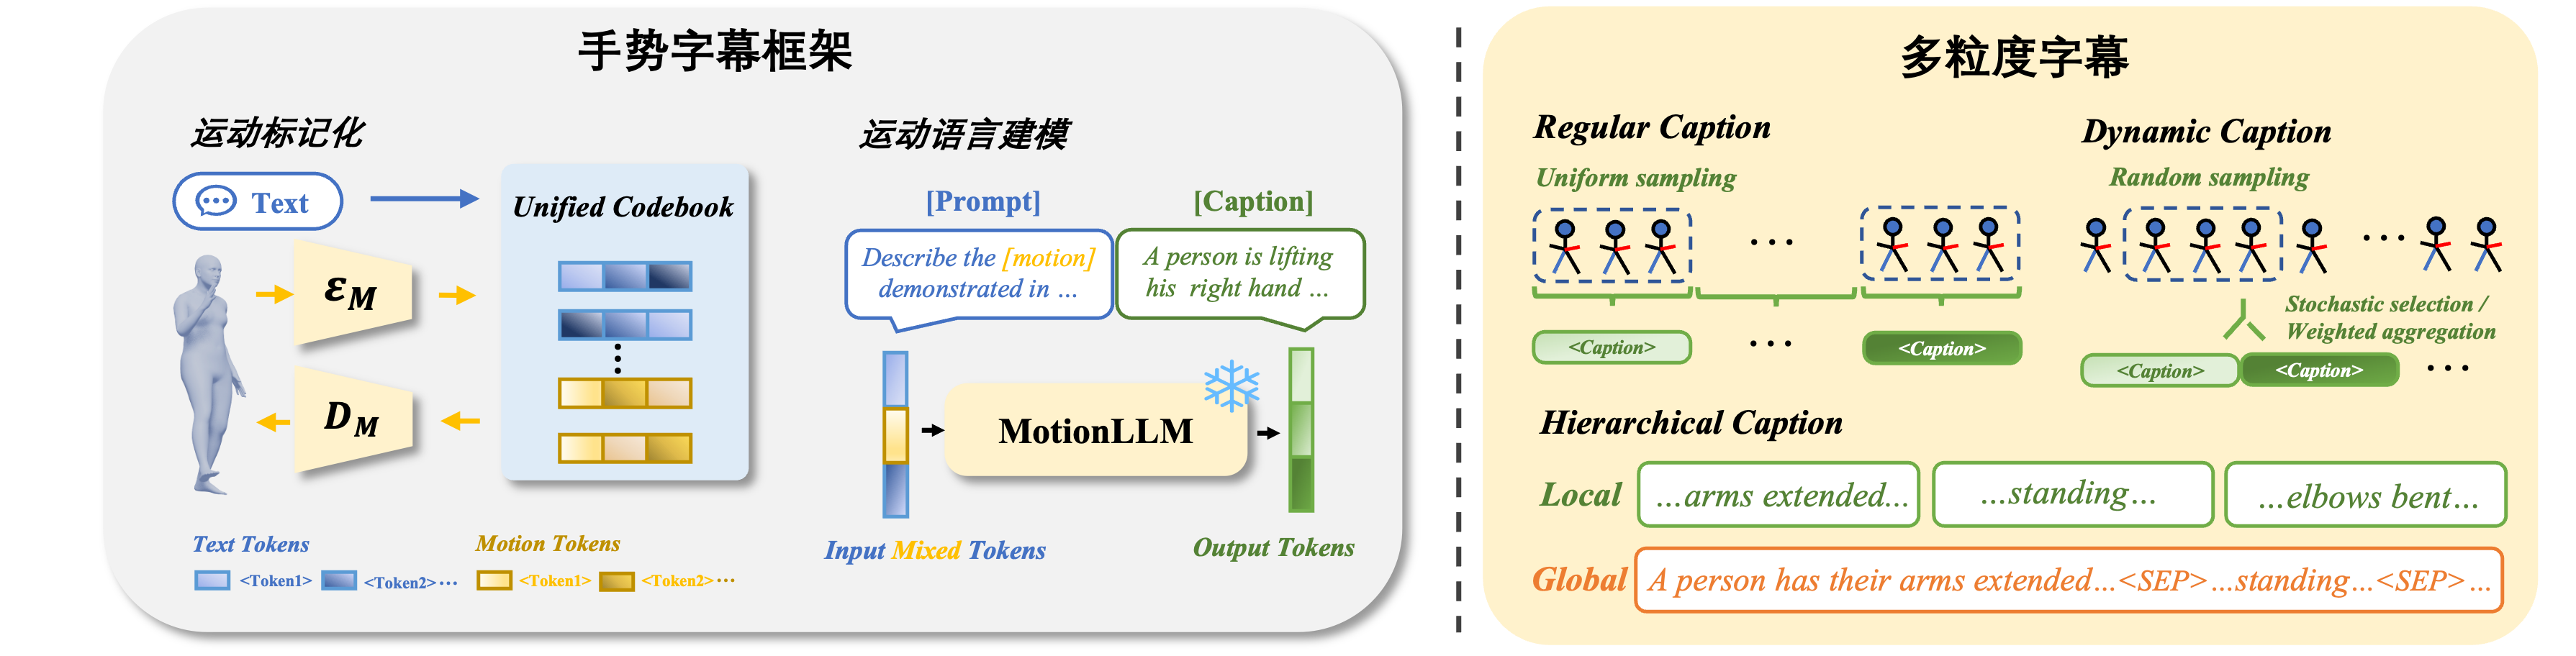
\includegraphics[width=\linewidth]{gesture_captioning_v1_zh.png}
  \caption{手势描述生成框架。我们的手势描述生成框架包含两个主要组件:
  运动分词器和运动感知语言模型。运动分词器将手势序列编码为离散的运动token序列,运动感知语
  言模型则基于这些token和提示模板生成对应的手势描述。}
  \label{fig:method:captioning}
\end{figure*}

\section{手势描述}
\label{sec:method:caption}
手势数据缺乏描述性文本标注显著限制了通过文本提示控制手势合成的能力~\cite{chen2024syntalker}。为了解决这个问题,我们提出了一种新颖的\textit{手势描述}方法,利用运动-语言模型为手势生成描述性标注。这种方法为手势数据集的语义标注稀缺问题提供了一个高效的解决方案,同时通过生成的描述实现精细的语义控制(详见第\ref{sec:method:control}节)。

我们的手势描述框架(图\ref{fig:method:captioning})包含两个主要组件:\textit{运动分词器}和\textit{运动感知语言模型(MotionLLM)}。
运动分词器基于~\cite{}中使用的VQ-VAE架构,由编码器$\mathcal{E_M}$和解码器$\mathcal{D_M}$组成,用于生成离散的运动令牌。
运动感知语言模型采用基于Transformer的架构,具有统一的文本-运动词表$\mathbf{V} = \{\mathbf{V_t}, \mathbf{V_m}\}$,使其能够在单个模型中灵活地联合建模文本和运动。
具体而言,手势序列首先转换为第\ref{sec:method:m_rep:unified}节中描述的统一运动表示,然后输入我们的手势描述框架。
给定一个包含M帧的手势运动序列$m^{1:M}=\{x^i\}^M_{i=1}$,运动分词器首先将其编码和量化为离散的运动令牌序列$z^{1:L}=\{z^i\}^L_{i=1}$。精心设计的\textit{提示模板}被分词为文本令牌$w^{1:N}=\{w^i\}^N_{i=1}$。随后,离散运动令牌和文本令牌被混合并共同输入运动感知语言模型,生成相应的手势描述$\hat{w}^{1:L}=\{w^i\}^L_{i=1}$。
在实践中,我们利用~\cite{jiang2024motiongpt}提供的预训练模型,并在推理过程中保持其参数冻结。
% TODO:可放补充材料
% 受限于MotionGPT所使用的人体运动数据集的格式,首先需要将手势表示转换为22关节的HumanML3D格式,然后输入到MotionGPT中生成描述。

\paragraph{实现细节}
表~\ref{tab:prompt_templates}展示了我们的手势描述框架中使用的提示模板集合。这些经过精心设计的模板会被多次随机采样,并与不同的手势片段配对以生成多样化的手势描述。这些模板的设计受到了最新运动-语言建模研究的启发~\cite{jiang2024motiongpt}。

此外,由于我们使用的MotionLLM是在22个关节点的人体运动数据集上预训练的,在进行描述生成推理之前,我们需要先将手势特征从$x\in \mathbb{R}^{T\times 659}$转换为$\mathbb{R}^{T\times 263}$的相似格式,这是通过仅保留前22个关节点的数据来实现的。这种转换不可避免地会导致一些细微的手指动作细节丢失。如果能有一个包含明确手指动作标注的更精细数据集,将能显著缓解这一局限性。

\begin{table*}[t]
\centering
\caption{手势描述框架中使用的提示模板示例。}
\footnotesize
\label{tab:prompt_templates}
\begin{tabular}{llc}
\toprule
Task & Input & Output \\
\midrule
\multirow{10}{*}{Gesture-to-Text} & Give me a summary of the motion being displayed in [motion] using words. & \multirow{10}{*}{[caption]} \\
& Explain the motion illustrated in [motion] using language. & \\
& Describe the action being represented by [motion] using text. & \\
& What kind of action is being demonstrated in [motion]? & \\
& Describe the movement demonstrated in [motion] in words. & \\
& Generate a sentence that explains the action in [motion]. & \\
& Please describe the movement depicted in [motion] using natural language. & \\
& Provide a description of the motion being displayed in [motion] using language. & \\
& Give me a brief summary of the movement depicted in [motion]. & \\
& Describe the movement demonstrated in [motion] using natural language. & \\
\bottomrule
\end{tabular}
\end{table*}

\section{多粒度描述控制}
\label{sec:method:control}
由于手势的时序动态性和语义信息的不同粒度,有效利用手势描述进行精确控制具有挑战性。为了解决这个问题,我们提出了一种\textit{多粒度手势控制机制},实现了跨多个时间和语义尺度的精细控制。

给定一个手势序列,我们将其分段为$m^{1:M}=\{m^{i:i+K-1}\}_{i=1}^{M-K+1}$,其中$K$表示分段长度。每个分段通过我们的手势描述框架生成\textit{局部描述}$\hat{w}^{1:L}=\{w^i\}^L_{i=1}$,同时通过用分隔符<SEP>连接局部描述形成\textit{全局描述}。基于这种分层描述结构,我们设计了三种互补的控制策略:
(1) \textit{常规控制}。该策略应用均匀时间分段生成局部描述,在保持时间一致性的同时实现对手势细节的精确控制。
(2) \textit{动态控制}。为了增强灵活性和鲁棒性,该策略在训练过程中引入可控的随机性。分段被随机采样,局部描述通过\textit{随机选择}(从候选描述中随机选择)或\textit{加权聚合}(基于时间重叠程度组合描述)进行装配。这种方法帮助模型学习处理不同的时间尺度和描述组合。
(3) \textit{分层控制}。在前述策略的基础上,我们将分层描述与分层条件注入(第\ref{sec:method:gld}节)相结合:局部描述、音频和时间步嵌入被串联并作为$c_1$注入去噪器编码器,确保与局部手势分段的精确语义和节奏同步;然后,全局描述作为$c_2$通过交叉注意力注入去噪器解码器,增强手势的整体连贯性和语义相关性。
这种多粒度控制机制在确保时间一致性的同时,实现了灵活的多尺度语义控制。



% 怎么使用text_audio(caption + speech)进行控制
% % 多粒度description control设计
% % 多模态condition融合方式,condition集成方式...

% 为了实现多尺度的精细描述,我们提出了多粒度的手势控制生成方式。
% 设计了3种控制方式:i) regular, 均匀分段装配局部描述 ii) dynamic,训练过程中随机采样分段,根据开始与结束帧,通过random选择或weighted加权装配局部描述 iii) hierarchical, 在局部描述的基础上,添加全局描述,并使用不同的condition注入方式:局部描述通过concat(Sec.~\ref{sec:method:gld})集成,注入transformer encoder进行self attention;随后,提取去噪隐向量$\hat{z}$作为query,全局描述作为key和value,注入transformer decoder,进行cross attention。
% 这样做的好处....(前期关注局部细节和语音节奏,后期通过全局语义进行指导增强)

\section{实验结果与分析}
\label{sec:experiments}
在本节中,我们通过定量和定性分析从四个方面评估我们的方法:
(1) \textbf{协同手势生成}。与最先进的基线相比,评估模型在联合语音和字幕控制下生成语音同步、语义相关的全身手势的能力。
(2) \textbf{文本驱动运动生成}。与最先进的文本到运动方法进行比较,以评估语义理解和非自发手势生成能力。
(3) \textbf{手势字幕}。评估生成的手势字幕的质量和多样性标志着弥合手势数据集中语义差距的第一种方法。
(4) \textbf{消融研究}。分析我们方法中关键组件的影响。

\subsection{实验设置}
\paragraph{数据集}
本文利用语音到手势数据集BEAT~\cite{liu2022beat}和文本到运动数据集HumanML3D~\cite{guo2022humanml3d}进行训练。这种跨数据集学习策略使我们能够引入额外的语义运动先验。
HumanML3D数据集包含14,616个基础运动序列和44,970个对应的文本描述,为运动生成任务提供了丰富的语义先验。
BEAT数据集包含约76小时的语音-手势对齐的多模态序列,涵盖了多样化的手势类型和说话场景,为语音驱动的手势生成提供了重要支持。
参照~\cite{liu2022beat},我们使用四位英语演讲者的手势数据。

\paragraph{评估指标}
我们从三个方面评估生成结果:
(1) 重建质量:使用抖动度和加速度指标~\cite{kucherenko2019analyzing}评估动作的平滑度和自然度。
(2) 语音到手势生成:使用FGD~\cite{yoon2020speech}评估身体手势的真实性。通过计算不同手势片段间的平均L1距离评估多样性~\cite{liu2024emage},使用BC评估语音与动作的同步性。
(3) 文本到运动生成:使用Frechet Inception Distance (FID)和Diversity (DIV)评估生成运动的真实性和多样性,使用motion-retrieval precision (R Precision)和Multi-modal Distance (MM Dist)评估运动与文本描述的匹配程度~\cite{chen2023executing}。

\paragraph{实现细节}
我们基于 Transformer 的 VAE 和降噪器 $\epsilon_\theta$ 均由编码器 $E$ 和解码器 $D$ 组成,每个包含 9 层和 4 个注意力头,具有 GELU 激活和残差连接。潜在维度设置为 $z \in \mathbb{R}^{1 \times 512}$。语义和音频嵌入都通过线性层投影到 512 维空间中,然后输入到降噪器中。
对于训练,我们使用 AdamW 优化器,学习率为 $1e^{-4}$,批处理大小为 128。VAE 训练了 6000 个 epoch,而扩散模型训练了 2000 个 epoch。在训练过程中,我们使用 1000 个扩散步骤和 50 个推理步骤,噪声方差 $\beta_t$ 从 $8.5 \times 10^{-4}$ 线性缩放到 0.012。在 VAE 阶段,KL 损失权重 $\beta$ 设置为 0.0001(公式~\ref{eq:loss_vae})。
在推理过程中,对于无分类器指导,音频和字幕指导比例默认设置为 $s_1=7$ 和 $s_2=1$,以平衡不同的条件贡献。

为平衡训练过程中不同数据集的数据分布,我们对数据加载器采用加权随机采样策略。
参照~\cite{yang2024freetalker},所有运动序列重采样至20 FPS,并截断或填充至180帧。对于HumanML3D数据集,仅使用长度在40至180帧之间的序列。

\begin{figure*}[t]
  \centering
  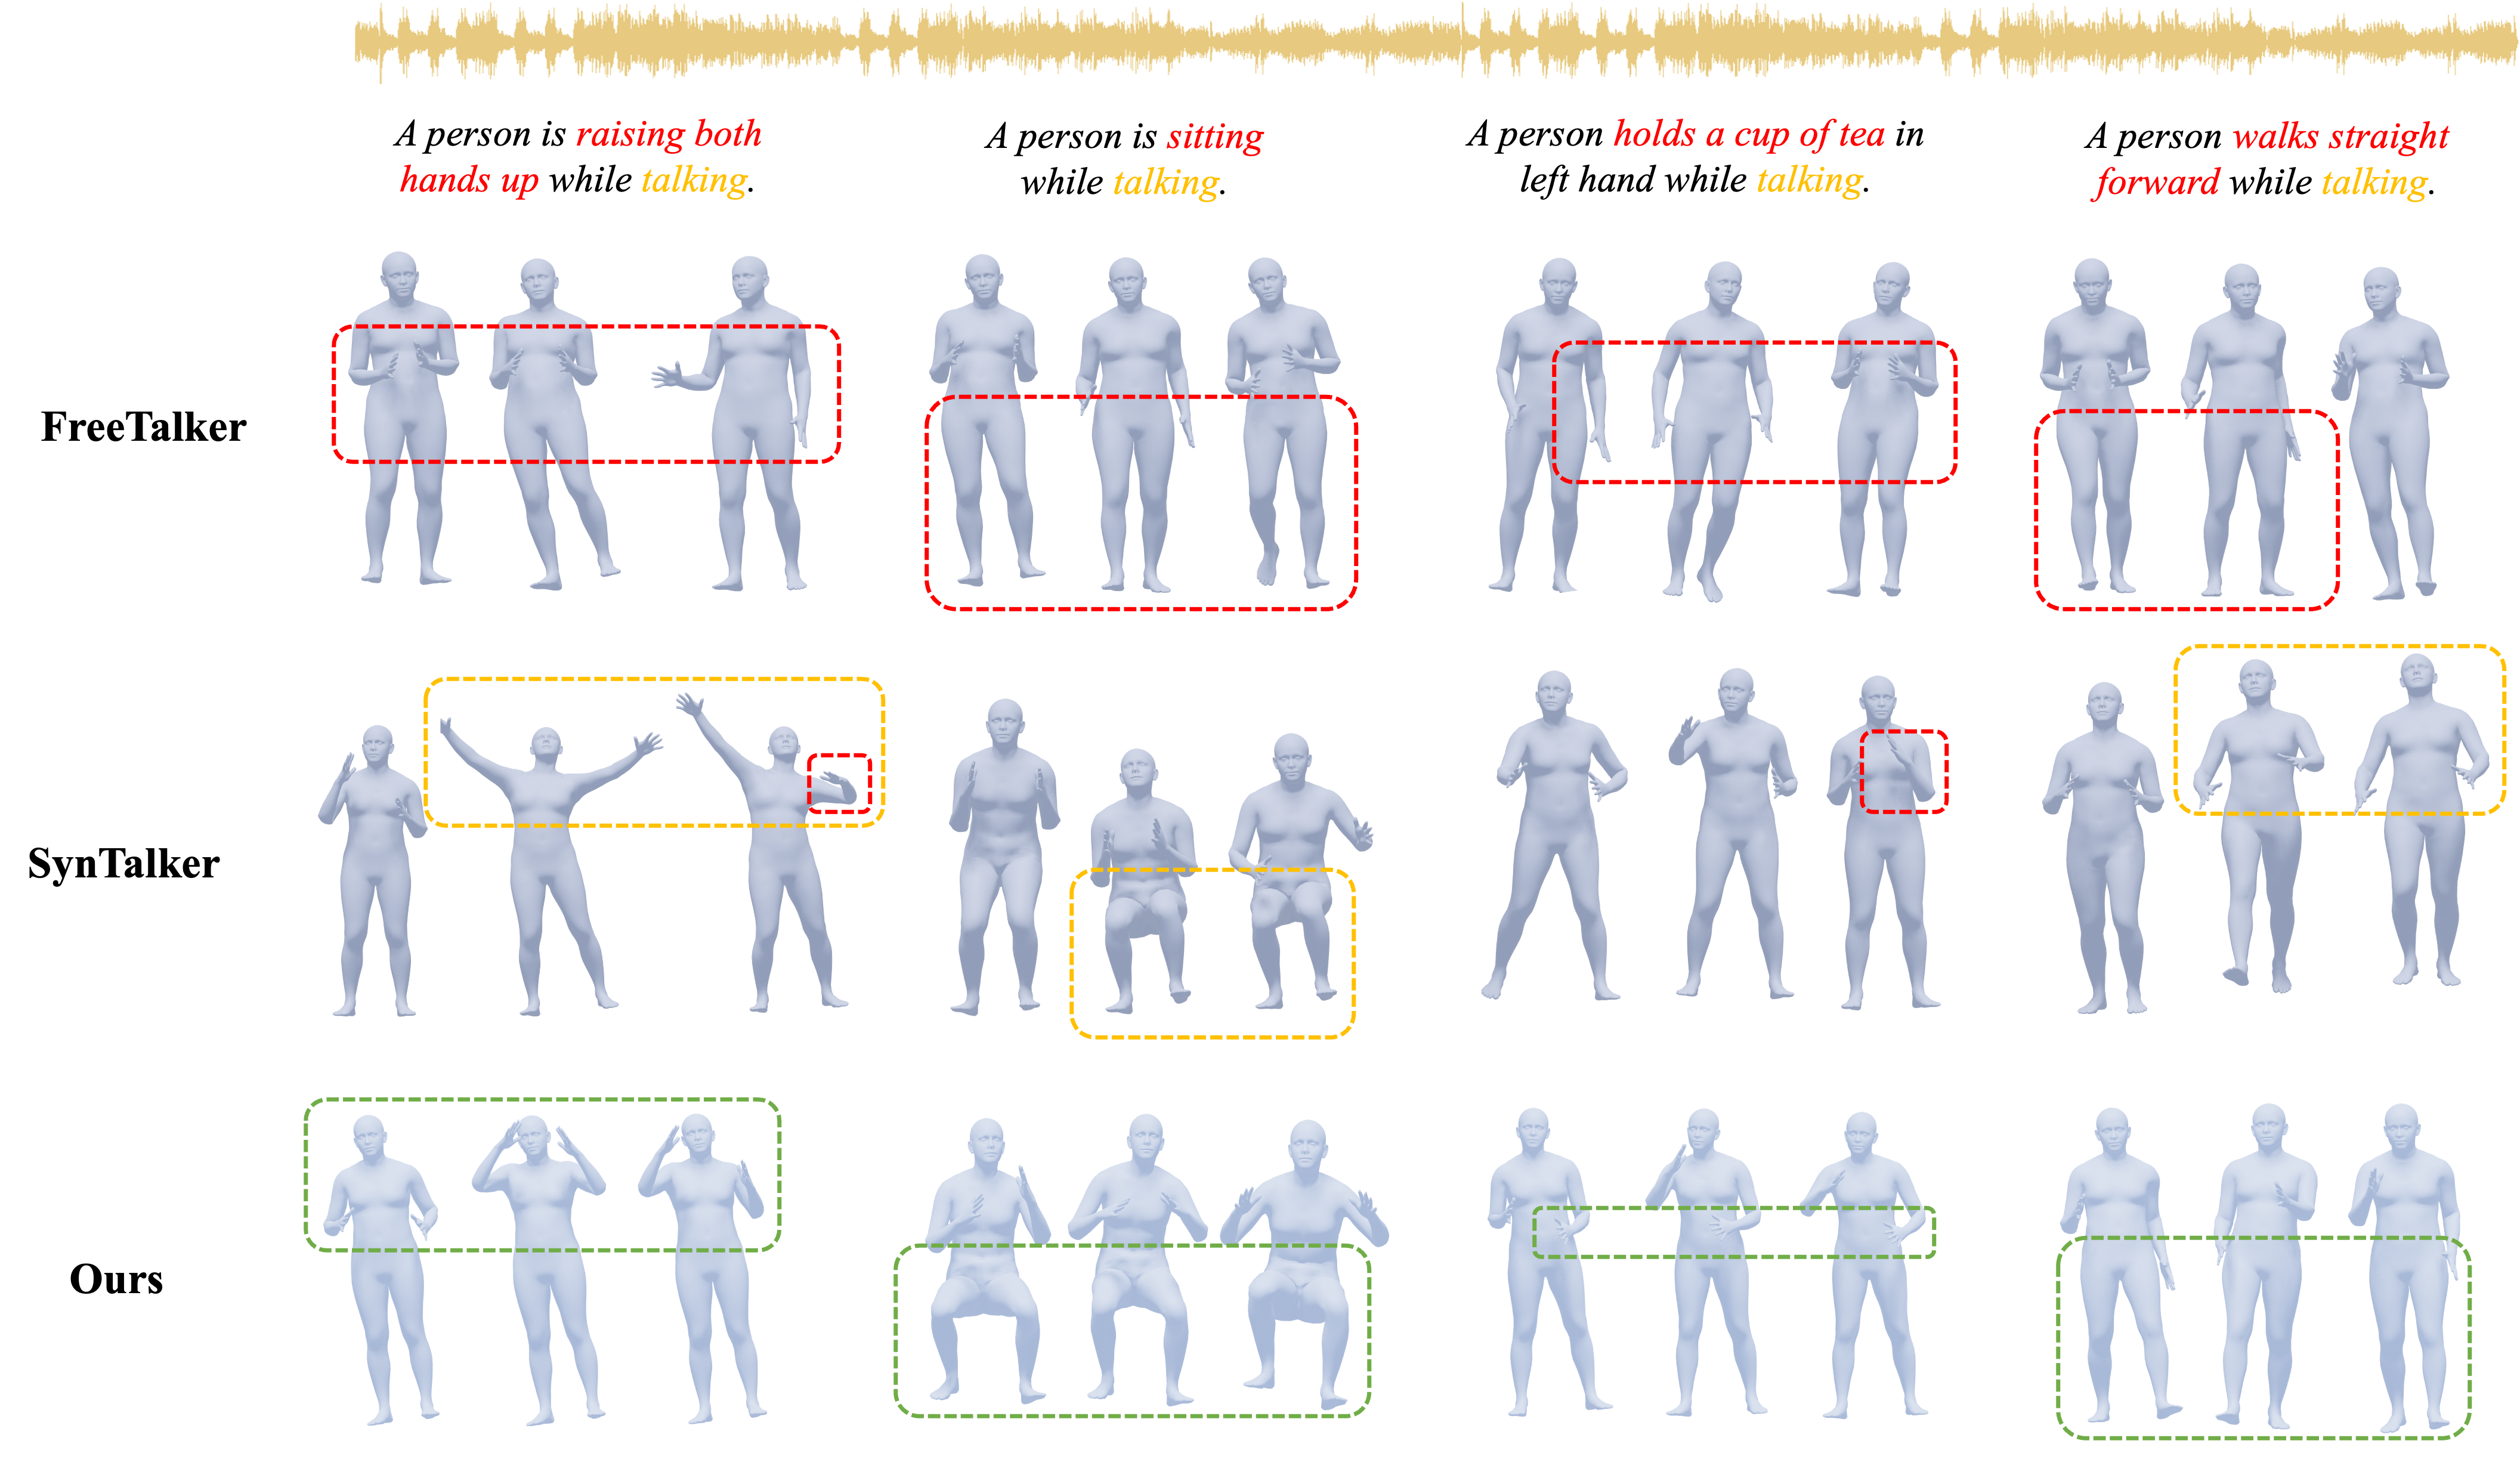
\includegraphics[width=\linewidth]{visualization_v1.png}
  \caption{协同手势生成的定性比较。 \textcolor{red}{红色} 框突出显示语义不一致,\textcolor[RGB]{204,153,0}{黄色} 框表示不自然的动作,\textcolor[RGB]{34,139,34}{绿色} 框表示协同良好的自然手势。}
  \label{fig:method:visualization}
\end{figure*}


\subsection{协同手势生成}
\subsubsection{定性对比}
我们首先评估我们的方法在生成协同的语音同步、语义相关的运动方面的表现。
如图~\ref{fig:method:visualization} 所示,我们将其与仅有的两部作品~\cite{yang2024freetalker,chen2024syntalker} 进行了比较,这两部作品都涉及相关的协同生成任务。
参照~\cite{chen2024syntalker},我们使用语音输入和四种不同的文本描述展示结果:\textit{``raising both hands up''}、\textit{``sitting''}、\textit{``holds a cup of tea''}和\textit{``walks straight forward''}。
结果表明,我们的方法有效地产生了节奏一致且语义一致的协同手势,同时实现了更自然的外观。
相比之下,FreeTalker 无法生成语义动作,而仅专注于语音驱动的手势。虽然 SynTalker 实现了一定的协同性,但它表现出细节上的不一致和不自然的僵硬性。
例如,在传达\textit{``holding ... in left hand''}时,我们的方法指示说话者将左手保持在腰部附近的稳定位置,这是FreeTalker和SynTalker结果中都缺失的细节。在表达\textit{``raising both hands up''}时,我们的方法通过同时抬起双臂保持与文本的一致性,而FreeTalker未能抬起双手,SynTalker则在举起后放下一只手。
此外,在表现\textit{``sitting''}和\textit{``walking straight forward''}时,我们的方法生成了更自然的说话者动作,相比之下SynTalker的结果显得较为僵硬。
值得注意的是,与 SynTalker 不同,我们的方法不需要额外的预训练或推理成本,并且可以实现更快的推理,如第~\ref{sec:exp_ablation}节所示。



% 主结果
\begin{table*}[t]
  \centering
  \caption{与基线模型和消融研究进行比较的定量结果。`$\rightarrow$' 表示越接近真实运动越好。每个指标均在 20 次运行的 95\% 置信区间下报告。我们报告 BC $\times 10^{-1}$ 和 Top-1 R-Precision。}
    % \small
    \footnotesize
    \label{tab:main_results}
    \begin{tabular}{l c@{\hspace{3pt}} c@{\hspace{3pt}} c@{\hspace{3pt}} c@{\hspace{3pt}} c@{\hspace{3pt}} c@{\hspace{3pt}} c@{\hspace{3pt}} c@{\hspace{3pt}} c}
    \toprule
    \multirow{3}{*}{Methods} & \multicolumn{2}{c}{Reconstruction} & \multicolumn{3}{c}{Audio-to-Gesture} & \multicolumn{4}{c}{Text-to-Motion} \\
    \cmidrule(lr){2-3} \cmidrule(lr){4-6} \cmidrule(lr){7-10}
    & Jerk$\rightarrow$ & Accel.$\rightarrow$ & FGD$\downarrow$ & BC$\uparrow$ & L1Div$\uparrow$ & FID$\downarrow$ & MM-Dist$\downarrow$ & Div$\rightarrow$ & R-Precision$\uparrow$ \\
    \midrule
    GT & $1.165^{\pm .000}$ & $0.043^{\pm .000}$ & - & - & - & - & $6.205^{\pm .043}$ & $5.512^{\pm .114}$ & $0.140^{\pm .008}$ \\
    Freetalker~\cite{yang2024freetalker} & $0.611^{\pm .013}$ & $0.030^{\pm .000}$ & $2.101^{\pm .026}$ & $1.147^{\pm .028}$ & $11.332^{\pm .025}$ & $0.761^{\pm .048}$ & $6.737^{\pm .051}$ & $5.396^{\pm .127}$ & $0.102^{\pm .008}$ \\
    Ours  & $1.190^{\pm .015}$ & $0.039^{\pm .001}$ & $3.173^{\pm .123}$ & $1.327^{\pm .049}$ & $10.861^{\pm .066}$ & $1.118^{\pm .061}$ & $6.814^{\pm .056}$ & $5.558^{\pm .126}$ & $0.100^{\pm .008}$ \\
    \midrule
    Ours-w/o mo. & $1.005^{\pm .014}$ & $0.032^{\pm .000}$ & $2.654^{\pm .041}$ & $2.627^{\pm .043}$ & $19.600^{\pm .089}$ & $3.911^{\pm .163}$ & $7.664^{\pm .050}$ & $4.070^{\pm .117}$ & $0.043^{\pm .004}$ \\
    % Ours-w/o cap. & $1.181^{\pm .011}$ & $0.039^{\pm .000}$ & $2.224^{\pm .074}$ & $2.330^{\pm .060}$ & $12.652^{\pm .109}$ & $1.041^{\pm .042}$ & $6.788^{\pm .056}$ & $5.414^{\pm .133}$ & $0.095^{\pm .008}$ \\
    Ours-w/o hcd.   & $1.201^{\pm .017}$ & $0.038^{\pm .001}$ & $2.302^{\pm .061}$ & $1.910^{\pm .004}$ & $12.781^{\pm .044}$ & $1.260^{\pm .063}$ & $6.872^{\pm .058}$ & $5.303^{\pm .107}$ & $0.102^{\pm .010}$ \\
    Ours-w/o mgc. & $1.239^{\pm .013}$ & $0.039^{\pm .000}$ & $3.123^{\pm .139}$ & $2.256^{\pm .045}$ & $15.363^{\pm .103}$ & $2.568^{\pm .099}$ & $7.031^{\pm .044}$ & $5.447^{\pm .150}$ & $0.082^{\pm .006}$ \\
  \bottomrule
  \end{tabular}
\end{table*}
\subsubsection{定量结果}
由于只有FreeTalker~\cite{yang2024freetalker}和SynTalker~\cite{chen2024syntalker}与本文工作研究范围相似,且SynTalker不支持多模态条件的定量评估方法,因此我们复现FreeTalker作为对比基线。

如表~\ref{tab:main_results}所示,我们的方法在所有评估指标中取得了可比或优越的结果,超过了Freetalker的重建质量,节拍一致性(BC $0.180\uparrow$),多样性(Div $0.162\uparrow$),同时维持有竞争力的文本匹配度。
值得注意的是,这些结果突出了我们方法在保持语音同步和语义相关性之间良好平衡的独特能力,证实了其在生成自然且可控的协同手势方面的有效性。



% 单条件结果 
\begin{table*}[t]
  \centering
  \caption{与 HumanML3D~\cite{guo2022humanml3d} 测试集上的最新方法进行比较。我们按照 \cite{chen2023executing} 计算标准度量。`$\rightarrow$' 表示越接近真实运动越好。每个度量均在 20 次运行的 95\% 置信区间下报告。}
  \label{tab:h3d_results}
  \small
  \begin{tabular}{l cccccc}
  \toprule
  \multirow{2}{*}{Methods} & \multirow{2}{*}{FID$\downarrow$} & \multirow{2}{*}{MM-Dist$\downarrow$} & \multirow{2}{*}{Div$\rightarrow$} & \multicolumn{3}{c}{R-Precision$\uparrow$} \\
  \cmidrule(lr){5-7}
  & & & & Top-1 & Top-2 & Top-3 \\
  \midrule
  GT  &  $0.001^{\pm .001}$ & $3.378^{\pm .007}$ & $10.471^{\pm .083}$ &  $0.490^{\pm .003}$ & $0.682^{\pm .003}$ & $0.783^{\pm .003}$ \\
  MDM~\cite{tevet2022mdm} & $1.390^{\pm .088}$ & $4.599^{\pm .037}$ & $10.704^{\pm .066}$ & $0.363^{\pm .007}$ & $0.553^{\pm .008}$ & $0.662^{\pm .007}$ \\
  T2M-GPT~\cite{zhang2023t2mgpt} &  $0.564^{\pm .012}$ & $3.867^{\pm .008}$ & $10.558^{\pm .083}$  & $0.433^{\pm .003}$ & $0.615^{\pm .002}$ & $0.716^{\pm .003}$ \\
  MLD~\cite{chen2023executing} & $0.963^{\pm .029}$ & $3.898^{\pm .012}$ & $10.401^{\pm .096}$ & $0.429^{\pm .003}$ & $0.613^{\pm .003}$ & $0.717^{\pm .002}$ \\
  MoMask~\cite{guo2024momask} & $0.222^{\pm .007}$ & $3.620^{\pm .011}$ & $10.621^{\pm .096}$ & $0.461^{\pm .002}$ & $0.657^{\pm .003}$ & $0.760^{\pm .002}$ \\
  SynTalker~\cite{chen2024syntalker} & $4.385^{\pm .034}$ & $4.499^{\pm .012}$ & $9.374^{\pm .073}$ & $0.375^{\pm .003}$ & $0.564^{\pm .003}$ & $0.681^{\pm .002}$ \\
  \midrule
  % Ours (w/o mo.rep.) & & & & & \\
  % Ours (w/o cap.)  & & & & &  \\
  % Ours  & $0.540^{\pm .013}$ & $6.833^{\pm .013}$ & $5.672^{\pm .154}$ & $0.104^{\pm .001}$ & $0.191^{\pm .002}$ & $0.270^{\pm .002}$ \\
  Ours  & $0.405^{\pm .012}$ & $3.584^{\pm .012}$ & $9.109^{\pm .235}$  & $0.424^{\pm .003}$ &$0.601^{\pm .003}$ & $0.702^{\pm .003}$ \\
  \bottomrule
  \end{tabular}
\end{table*}

\subsection{文本驱动的运动生成}
\label{sec:exp_t2m}
我们进一步将我们的方法与最先进的文本到运动方法进行比较,以验证其在捕获语义和生成非自发运动方面的能力。
为了公平比较,我们仅使用文本条件报告 HumanML3D 测试集的结果。
表格~\ref{tab:h3d_results} 显示,与 SOTA 模型相比,我们的方法实现了高级性能,实现了最佳文本对齐(MM-Dist 3.584)和第二好的生成保真度(FID 0.405)。这强调了我们的分层控制降噪器在集成细粒度语义方面的有效性。
值得注意的是,我们的方法明显优于类似的协同方法 SynTalker~\cite{chen2024syntalker},突出了其在协同生成和增强语义控制方面的优势。


\begin{figure*}[t]
  \centering
  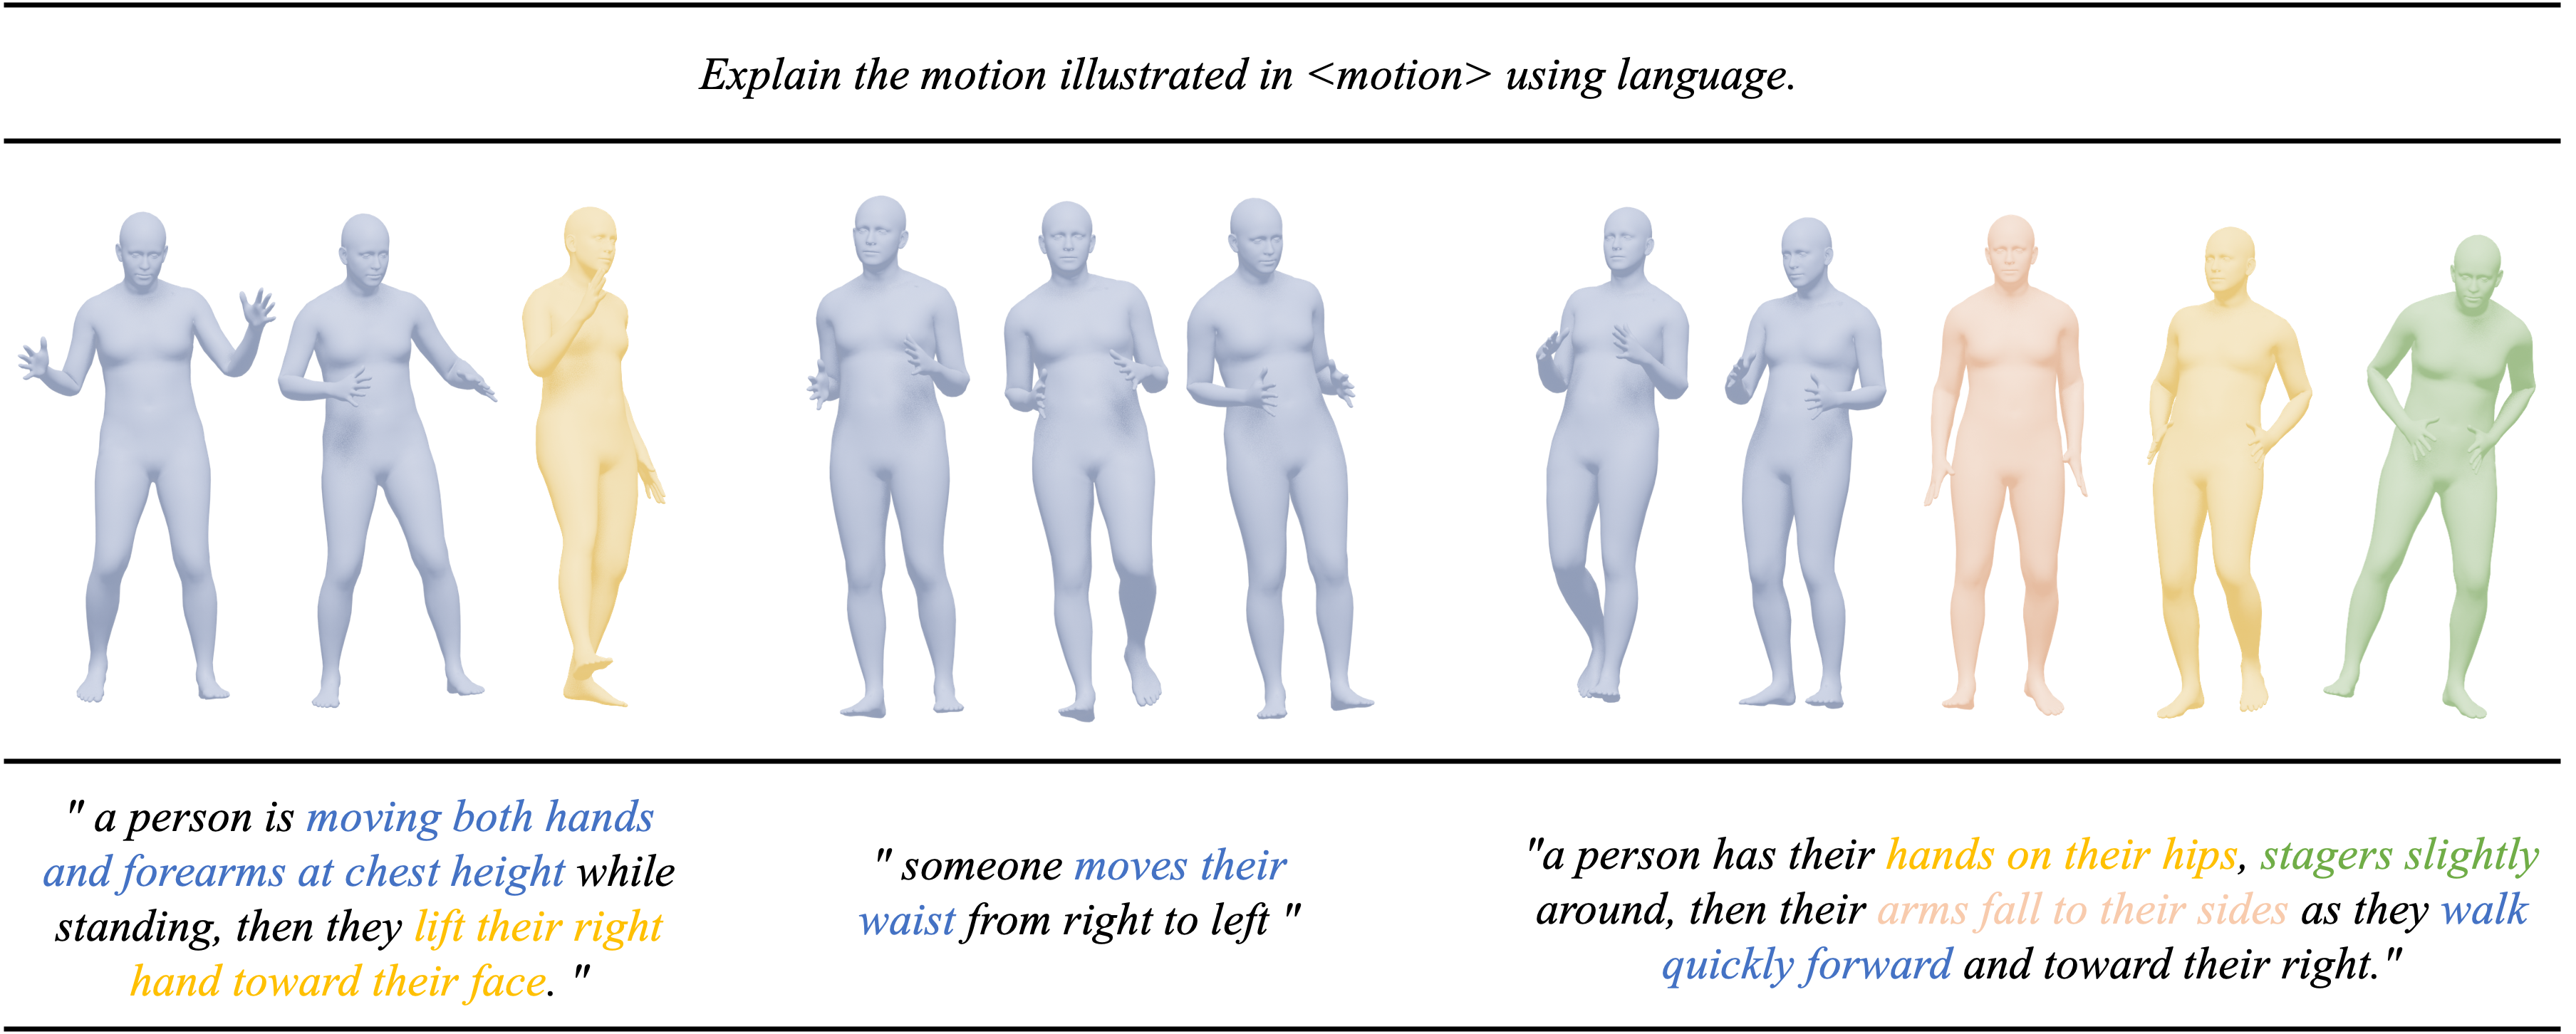
\includegraphics[width=\linewidth]{visualization_caption_v1.png}
  \caption{手势描述生成结果示例。生成的描述准确地描述了整体运动模式和细粒度的手势细节。}
  \label{fig:visualization_caption}
\end{figure*}
\subsection{手势描述生成}
如图~\ref{fig:visualization_caption}所示,所提出的手势描述框架展示了在生成描述性手势标注方面的实用能力。
结果表明,我们的方法不仅能准确描述手势运动分布内的细粒度手部动作(如\textit{``moving both hands and forearms at chest height''}),还能捕捉粗粒度的全身动作(如\textit{``moves their waist from ..."})。
此外,由于手势运动通常持续较长时间,所提出的多粒度描述方法在捕捉长时间窗口内的连续复杂组合动作方面表现出优势(如\textit{``a person \textless motion 1\textgreater, then \textless motion 2\textgreater as \textless motion 3\textgreater''})。
然而,我们也注意到对于较长的手势序列,模型在时序位置感知方面存在困难,偶尔会混淆动作顺序。这一限制可以通过使用我们提出的细粒度描述策略来管理动作复杂度。未来的改进可能涉及引入更强的位置编码或时序建模。

\begin{figure}[t]
    \centering
    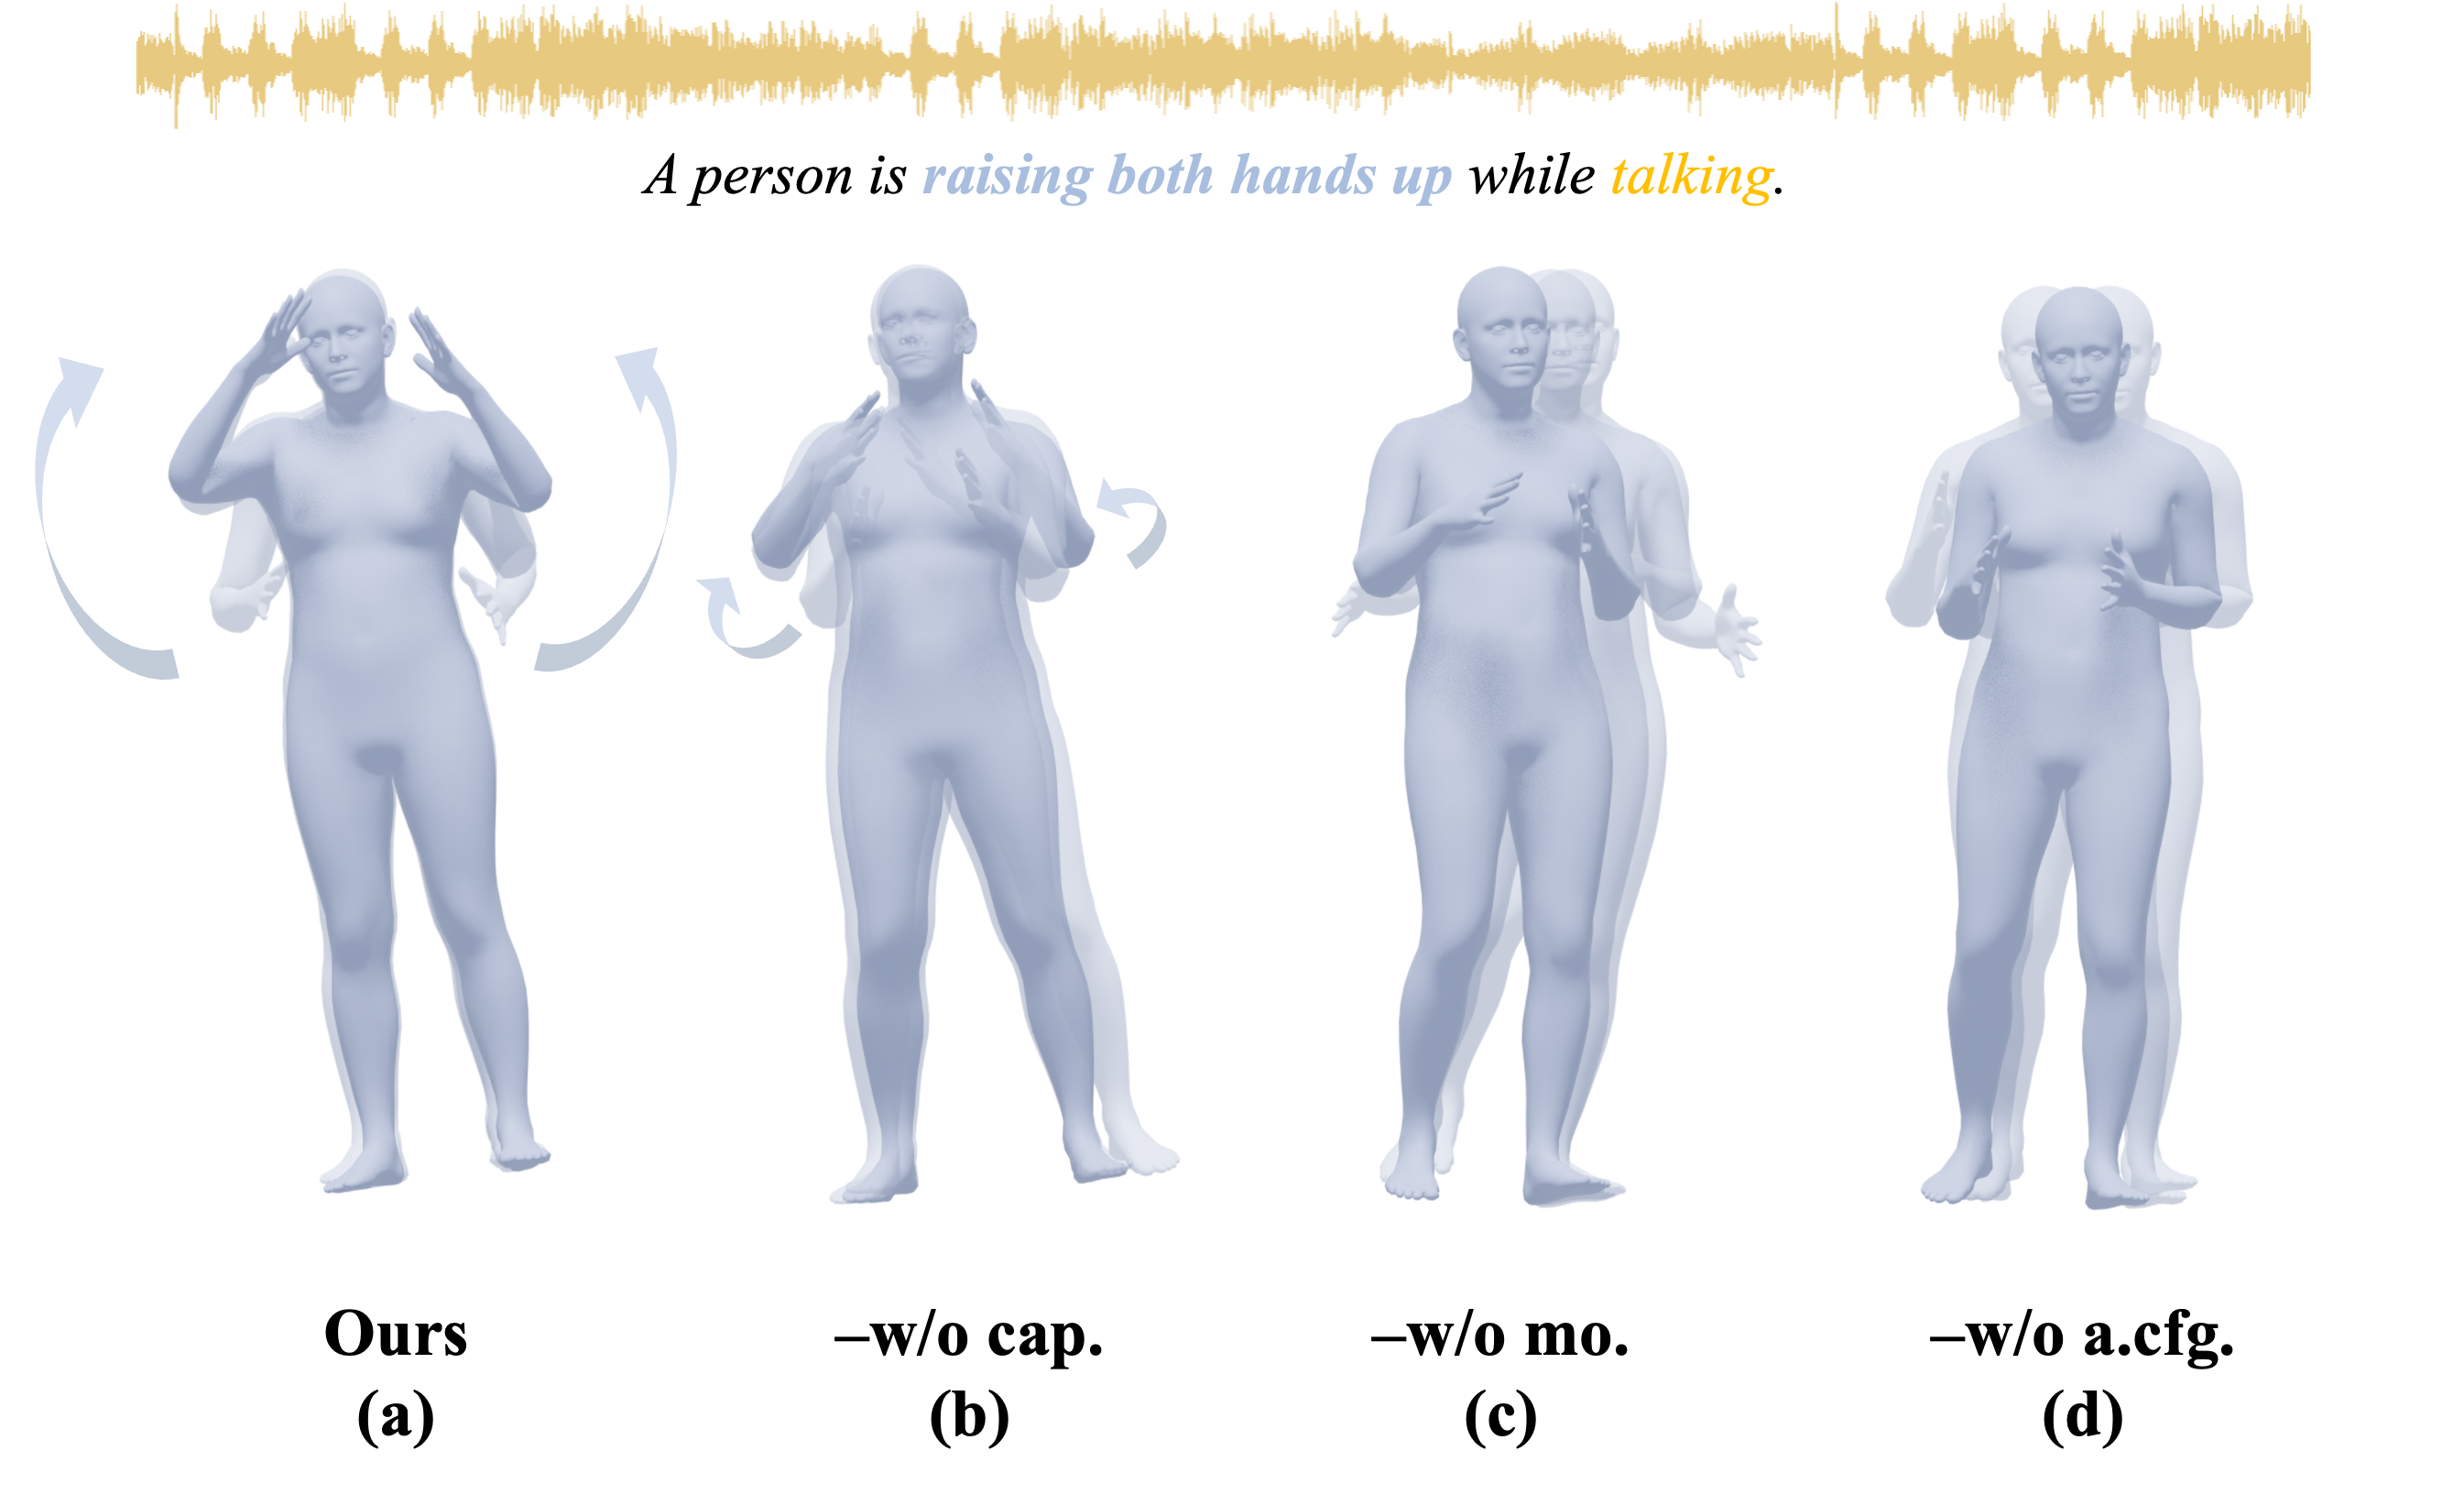
\includegraphics[width=0.7\linewidth]{ablation.png}
    \caption{定性消融研究。结果是使用语音音频和单字幕 \textit{``A person is raising both hands up while talking''} 生成的。}
    \label{fig:ablation}
\end{figure}

\subsection{消融实验}
\label{sec:exp_ablation}
为了进一步评估不同组件对协同生成的影响,我们在此任务下进行了消融研究。
定量结果如表~\ref{tab:main_results} 所示,定性结果如图~\ref{fig:ablation} 所示。我们使用音频和单个字幕条件 (\textit{``A person is raising both hands up while talking''}) 进行了定性评估。
如图~\ref{fig:ablation}(a) 所示,我们的完整模型有效地捕捉了音频节奏和语义指令,生成自发的语音手势,同时遵循字幕指导产生非自发的手势(向上举起双手)。

\paragraph{手势描述}
图~\ref{fig:ablation}(b)展示了移除手势描述后的影响。没有描述的语义指导,模型只能生成与语音同步的基本协同手势,无法产生有意义的非自发运动。
这表明手势描述在提供语义指导和补充缺失的手势文本标注方面发挥着关键作用。

\paragraph{统一运动表示}
移除统一的运动表征(图\ref{fig:ablation}(c))显著限制了模型生成除典型同语动作之外的多样且语义上有意义的手势的能力。虽然细微的向上手部动作仍然存在,但说话者未能完全执行标题中描述的举起双手的预期手势。
表~\ref{tab:main_results}(\textit{Ours-w/o mo.})中的定量结果进一步证实了这种退化,显示语义相关性大幅下降,反映在明显更差的 FID($2.793\uparrow$)、MM-Dist($0.850\uparrow$)和 R-Precision(Top-1 $0.057\uparrow$)中。

\paragraph{分层控制降噪器} % [定量] 包括denoiser设计,condition集成方式
如表~\ref{tab:main_results}所示,删除分层控制的降噪器(\textit{Ours-w/o hcd.})会导致重建质量下降(Jerk $0.011\uparrow$)和条件协同性减弱。具体而言,该模型表现出更强的偏向于重建同语手势(BC $0.583\uparrow$),同时无法保持语义相关性(MM-Dist $0.058\uparrow$)。这些发现强调了我们的分层控制降噪器在确保有效的多模态条件协同方面的关键作用。

\paragraph{多粒度字幕}
如表~\ref{tab:main_results} 所示,删除多粒度字幕(\textit{Ours-w/o mgc.})会导致生成的手势的语义相关性显著下降。这凸显了我们的多粒度字幕机制在促进精确和上下文感知的语义注入方面的重要性。在这种情况下,音频作为初始条件,而本地字幕提供精细条件。

\paragraph{多模态无分类器指导}
图~\ref{fig:ablation}(d)展示了仅对文本模态应用无分类器指导的效果。
由于训练时缺乏语音模态的无条件指导,模型在推理时难以融合多模态信号,过度依赖语音输入,导致手势多样性有限且语义对齐性差。
这些发现突显了组合多模态指导在实现平衡手势生成中的重要性,有助于整合语音节奏和语义约束。

\begin{table*}[t]
    \centering
    \caption{多粒度字幕策略的消融研究。``Reg.'' 表示常规字幕策略,``Dyn.'' 表示动态字幕策略,``Hie.'' 表示分层字幕策略。
    每个指标均在 20 次运行的 95\% 置信区间下报告。我们报告 BC $\times 10^{-1}$ 和 Top-1 R-Precision。}
    \footnotesize
    \label{tab:ablation}
    \begin{tabular}{l c@{\hspace{3pt}} c@{\hspace{3pt}} c@{\hspace{3pt}} c@{\hspace{3pt}} c@{\hspace{3pt}} c@{\hspace{3pt}} c@{\hspace{3pt}} c@{\hspace{3pt}} c}
    \toprule
    \multirow{3}{*}{Methods} & \multicolumn{2}{c}{Reconstruction} & \multicolumn{3}{c}{Audio-to-Gesture} & \multicolumn{4}{c}{Text-to-Motion} \\
    \cmidrule(lr){2-3} \cmidrule(lr){4-6} \cmidrule(lr){7-10}
    & Jerk$\rightarrow$ & Accel.$\rightarrow$ & FGD$\downarrow$ & BC$\uparrow$ & L1Div$\uparrow$ & FID$\downarrow$ & MM-Dist$\downarrow$ & Div$\rightarrow$ & R-Precision$\uparrow$ \\
    \midrule
    GT & $1.165^{\pm .000}$ & $0.043^{\pm .000}$ & - & - & - & - & $6.205^{\pm .043}$ & $5.512^{\pm .114}$ & $0.140^{\pm .008}$  \\
    \midrule
    Ours-Reg.  & $1.201^{\pm .017}$ & $0.038^{\pm .001}$ & $2.302^{\pm .061}$ & $1.910^{\pm .004}$ & $12.781^{\pm .044}$ & $1.260^{\pm .063}$ & $6.872^{\pm .058}$ & $5.303^{\pm .107}$ & $0.102^{\pm .010}$  \\
    Ours-Dyn.  & $1.189^{\pm .013}$ & $0.038^{\pm .000}$ & $2.866^{\pm .106}$ & $1.943^{\pm .037}$ & $14.471^{\pm .110}$ & $1.404^{\pm .049}$ & $6.955^{\pm .044}$ & $5.440^{\pm .114}$ & $0.095^{\pm .006}$  \\
    Ours-Hie.  & $1.190^{\pm .015}$ & $0.039^{\pm .001}$ & $3.173^{\pm .123}$ & $1.327^{\pm .049}$ & $10.861^{\pm .066}$ & $1.118^{\pm .061}$ & $6.814^{\pm .056}$ & $5.558^{\pm .126}$ & $0.100^{\pm .008}$ \\
    \bottomrule
    \end{tabular}
\end{table*}

\paragraph{多粒度描述控制}
表~\ref{tab:ablation}进一步展示了本文方法在不同粒度描述控制策略下的性能。
分层控制策略(分层控制)在所有指标上实现了最优平衡:与常规和动态控制策略相比,它表现出更好的语义相关性(MM-Dist更低,$6.814$ vs $6.872$和$6.955$)、更好的运动质量(FID降低11.3\%和25.6\%),同时有效维持了语音同步性和运动多样性。
此外,动态策略在协同手势同步性(BC: $1.943$)和多样性(L1Div: $14.471$)方面表现出优势,这可能归因于其自适应采样机制增强了训练数据的多样性,使模型能够产生更丰富的节奏手势模式。
这些综合结果表明,我们的多粒度描述控制策略有效协同了多模态信号,在运动自然度、语音同步性和语义对齐性之间实现了平衡的权衡。分层控制策略在细粒度语义注入方面表现尤为出色,导致生成手势具有更强的语义相关性。

\paragraph{推理时间}
尽管扩散模型表现出色,但其较长的推理时间仍是主要瓶颈。
为评估推理效率,我们在单个NVIDIA RTX 3090 GPU上测量每句平均推理时间(AITS)~\cite{chen2023executing},批量大小设为1,不包括模型加载时间。
结果显示我们的方法实现了 $0.842^{\pm .002}$ 秒的AITS,比FreeTalker~\cite{yang2024freetalker} ($6.632^{\pm .044}$s) 和 SynTalker~\cite{chen2024syntalker} ($5.804^{\pm .044}$s) 快6倍以上。
这种显著的加速可以归因于我们高效的分层去噪架构和优化的潜在扩散过程,使我们的方法更适合实际应用。

\subsection{更多可视化结果}
\paragraph{更多协同生成结果}
如图~\ref{fig:vis_supply}所示,我们使用相同的音频和不同的文本标题提供了更加协同的生成结果。
这些结果进一步证实了我们提出的方法在联合语音字幕控制下生成协同语音自发手势和字幕驱动的非自发运动的有效性。

% 更多手势字幕结果
\paragraph{更多手势字幕结果}
我们在图.~\ref{fig:vis_caption_supply}中展示了额外的手势字幕结果,进一步证明了我们的方法在准确地将手势映射到文本方面的有效性。
正如彩色框中突出显示的那样,该模型在描述复杂、连续的动作时成功捕捉了细粒度的手部动作和粗粒度的全身动作。

\begin{figure*}[t]
  \centering
  \includegraphics[width=\linewidth]{visualization_supply.png}
  \caption{协同手势生成的更多视觉结果。}
  \label{fig:vis_supply}
\end{figure*}

\begin{figure*}[t]
  \centering
  \includegraphics[width=\linewidth]{visualization_caption_supply.png}
  \caption{更多手势字幕结果。彩色框突出显示了手势和文本字幕之间的精确映射。}
  \label{fig:vis_caption_supply}
\end{figure*}


\section{本章小结}
本章提出了一种基于描述驱动的协同手势生成框架(CoordSpeaker),旨在解决手势生成中的语义标注缺失和多模态协同控制挑战。
首先,第~\ref{sec:method:m_rep}节引入了统一的运动表示方法,通过将不同来源的运动数据映射到紧凑的潜在空间,为跨数据集手势生成奠定基础。
随后,第~\ref{sec:method:gld}节提出了可控手势潜在扩散模型,该模型通过手势VAE学习紧凑的潜在表示,并利用分层条件扩散模型实现高效的多模态条件生成。
为了解决手势数据缺乏描述性文本标注的问题,第~\ref{sec:method:caption}节设计了一个手势描述框架,利用动作-语言模型为手势数据生成语义标注。
第~\ref{sec:method:control}节提出的多粒度描述控制机制进一步增强了对生成过程的精确控制。
最后,第~\ref{sec:experiments}节通过大量定性与定量实验验证了本文方法的有效性。
大量实验表明,本文方法不仅能生成语义连贯、节奏同步的协同手势动作,而且在推理效率上相比现有方法提升了6倍以上,展现了在实际应用中的潜力。
